\documentclass[11pt, aspectratio=169]{beamer}
  % papersize={16cm,9cm},

\newcommand{\formula}{F}
\newcommand{\Obj}{\textsc{O}}
\newcommand{\inc}{\text{I}}
\newcommand{\dec}{\text{D}}
\newcommand{\var}{\textsc{var}}
\newcommand{\lit}{\textsc{lit}}
\newcommand{\Min}{\texttt{Minimize-\allowbreak{}Inc}}
\newcommand{\Simpr}{\texttt{Solution-\allowbreak{}Improving-\allowbreak{}Search}}
\newcommand{\E}{\texttt{EnumSols}}
\newcommand{\Ex}{\texttt{ExistsSol}}
\newcommand{\T}{\mathtt{T}}
\newcommand{\assumps}{\mathcal{A}}
\newcommand{\satsolver}{\texttt{isSAT}}
\newcommand{\res}{\text{res}}
\newcommand{\algname}{\textsc{BiOptSat}}
\newcommand{\tot}{\textsc{Tot}}
\newcommand{\ov}[2]{\langle #1 < #2 \rangle}
\newcommand{\ove}[2]{\langle #1 \leq #2 \rangle}
\newcommand{\satunsat}{\texttt{SAT-\allowbreak{}UNSAT}}
\newcommand{\unsatsat}{\texttt{UNSAT-\allowbreak{}SAT}}
\newcommand{\msu}{\texttt{MSU3}}
\newcommand{\I}{\mathcal{I}}
\newcommand{\Act}{\texttt{Act}}
\newcommand{\oll}{\texttt{OLL}}
\newcommand{\msh}{\texttt{MSHybrid}}
\newcommand{\hs}{\texttt{hs}}
\newcommand{\nsamp}{n}
\newcommand{\nfeat}{m}
\newcommand{\nclauses}{k}
\newcommand{\selector}{s}
\newcommand{\noise}{\eta}
\newcommand{\equals}{e}
\newcommand{\nelems}{n}
\newcommand{\nsets}{m}
\newcommand{\setcard}{s}
\newcommand{\elemprob}{p}
\newcommand{\sets}{\mathcal{S}}
\newcommand{\element}{e}
\newcommand{\cover}{\mathcal{C}}
\newcommand{\cost}{c}
\newcommand{\cores}{\mathcal{K}}
\newcommand{\core}{\kappa}
\newcommand{\sol}{\tau}
\newcommand{\scep}{SetCovering-EP}
\newcommand{\scsc}{SetCovering-SC}
\newcommand{\clause}{C}
\newcommand{\softs}{\textsc{S}}
\newcommand{\generalobj}{f}
\newcommand{\nobj}{p}
\newcommand{\feasible}{\mathcal{X}}
\newcommand{\decvar}{x}
\newcommand{\soloone}{\{i_2,\allowbreak d_1,\allowbreak d_3,\allowbreak d_4,\allowbreak \lnot i_1,\allowbreak \lnot i_3,\allowbreak \lnot i_4,\allowbreak \lnot d_2\}}
\newcommand{\solotwo}{\{i_1,\allowbreak i_2,\allowbreak d_1,\allowbreak d_2,\allowbreak \lnot i_3,\allowbreak \lnot i_4,\allowbreak \lnot d_3,\allowbreak \lnot d_4\}}
\newcommand{\solothree}{\{i_2,\allowbreak d_1,\allowbreak d_3,\allowbreak d_4,\allowbreak \lnot i_1,\allowbreak \lnot i_3,\allowbreak \lnot i_4,\allowbreak \lnot d_2\}}
\newcommand{\solcone}{\{i_1,\allowbreak i_2,\allowbreak i_3,\allowbreak i_4,\allowbreak d_1,\allowbreak d_2,\allowbreak d_3,\allowbreak d_4\}}
\newcommand{\solctwo}{\{i_1,\allowbreak i_2,\allowbreak d_1,\allowbreak d_2,\allowbreak d_3,\allowbreak d_4,\allowbreak \lnot i_3,\allowbreak \lnot i_4\}}
\newcommand{\solcthree}{\{i_2,\allowbreak d_1,\allowbreak d_2,\allowbreak d_3,\allowbreak d_4,\allowbreak \lnot i_1,\allowbreak \lnot i_3,\allowbreak \lnot i_4\}}
\newcommand{\solcfour}{\{i_1,\allowbreak i_2,\allowbreak i_3,\allowbreak d_1,\allowbreak d_2,\allowbreak \lnot i_4,\allowbreak \lnot d_3,\allowbreak \lnot d_4\}}
\newcommand{\solmcstrap}{\{i_1,\allowbreak i_3,\allowbreak i_4,\allowbreak d_1,\allowbreak d_3,\allowbreak d_4,\allowbreak \lnot i_2,\allowbreak \lnot d_2\}}
\newcommand{\TODO}[1]{\textcolor{red}{#1}}
\newcommand{\thr}{\texttt{thr}}
\newcommand{\NP}{$\mathcal{NP}$}

\mode<presentation>{}

%%%%%%%%%%%%%%%%%%%%%%%%%%%%%%
% Fill in the following information: AUTHOR, TITLE, DATE

\author{Christoph Jabs}
\title[\algname{}]{MaxSAT-Based Bi-Objective Boolean Optimization}
\date{10th April 2022}
\institute{HIIT, Department of Computer Science, University of Helsinki}

%%%%%%%%%%%%%%%%%%%%%%%%%%%%%%
% load packages
% add packages if needed

\usepackage[T1]{fontenc}
\usepackage[british]{babel}
\usepackage{amsmath,amsfonts,amssymb,amsthm}
\usepackage{color}
\usepackage[tracking=smallcaps, letterspace=-55]{microtype} % package for font spacing

\usepackage{transparent} % for setting opacity of pictures
\usepackage{pifont} % for checkmark (\ding{51}) and cross (\ding{55})
\usepackage{booktabs,array} % for tables
\usepackage{graphicx} % for figures
\graphicspath{{./img}} % to set the path of figures
\usepackage{algorithm}       % For pseudocode
\usepackage[noend]{algorithmic} % For pseudocode
\usepackage{appendixnumberbeamer}
\usepackage{cancel}
\usepackage{tikz}


%%%%%%%%%%%%%%%%%%%%%%%%%%%%%%
% set beamer colors

\definecolor{hyblue}{RGB}{0,155,255}
\setbeamercolor{alerted text}{fg=hyblue}
\setbeamercolor{structure}{fg=hyblue}

\setbeamertemplate{itemize item}{\color{hyblue}}

%%%%%%%%%%%%%%%%%%%%%%%%%%%%%%
% set font (helvetica plays the role of Arial)
\usepackage{helvet}
\renewcommand{\familydefault}{\sfdefault}

%%%%%%%%%%%%%%%%%%%%%%%%%%%%%%
% set frametitle

\setbeamercolor{frametitle}{fg=black}%{fg=hyblue}
\setbeamerfont{frametitle}{series=\bfseries, shape=\scshape, size=\huge}
\setbeamertemplate{frametitle}[default][left,leftskip=3.5cm] % left shift of frame title
\addtobeamertemplate{frametitle}{\vspace{0.5cm}}{\vspace{1cm}} % spacing above and below frame title

%%%%%%%%%%%%%%%%%%%%%%%%%%%%%%
% set footline and headline
\beamertemplatenavigationsymbolsempty
\setbeamertemplate{headline}{ }
\setbeamertemplate{footline}{%
	 \usebeamercolor[fg]{page number in head/foot}%
	 \usebeamerfont{page number in head/foot}%
	\hspace{0.5cm}	
	
\includegraphics[width=2.5cm]{HY__LC05_txt__L_3L_B3____BW_cropped}
	\hfill
	\insertshorttitle\ /\ \insertshortauthor	\hfill
	\insertshortdate	\hspace{0.5cm}
	\insertframenumber\,/\,\inserttotalframenumber \hspace{0.5cm} \vskip2pt%
}

%%%%%%%%%%%%%%%%%%%%%%%%%%%%%%
% Other style settings
\useinnertheme{circles}

%%%%%%%%%%%%%%%%%%%%%%%%%%%%%%
%%%%%%%%%%%%%%%%%%%%%%%%%%%%%%

\definecolor{color0}{RGB}{64,83,211}
\definecolor{color1}{RGB}{221,179,16}
\definecolor{color2}{RGB}{181,29,20}
\definecolor{color3}{RGB}{0,190,255}
\definecolor{color4}{RGB}{251,73,176}
\definecolor{color5}{RGB}{0,178,93}
\definecolor{color6}{RGB}{202,202,202}

\newcommand<>{\xxcancel}[1]{\alt#2{\xcancel{#1}\vphantom{#1}}{#1}}

\begin{document}

{
\usebackgroundtemplate{
\setlength{\unitlength}{1cm}
\begin{picture}(16,9)
	\put(-0.1,5){ 
\includegraphics[width=4cm]{HY__LA01_Flame_____B3____BW} }
\end{picture}
\setlength{\unitlength}{1pt}
}
\setbeamertemplate{headline}{ }%
\begin{frame}[noframenumbering]{}
\vspace{2.5cm}
\begin{center}
\huge
\textcolor{hyblue}{ \bf
\inserttitle
} \\
{\large
\insertauthor}
\end{center}
\end{frame}
}

\usebackgroundtemplate{
\setlength{\unitlength}{1cm}
\begin{picture}(16,2.5)
\put(0.1,0){

\includegraphics[width=2.5cm]{HY__LA01_Flame_____B3____BW}\hfill
}
\end{picture}
\setlength{\unitlength}{1pt}
}

\begin{frame}{Introduction}
  % Outline of the presentation
  % Paper under review for SAT 2022
  \begin{columns}
    \begin{column}{0.55\textwidth}
      {\LARGE
      MaxSAT-Based Bi-Objective Boolean Optimization
      }
    \end{column}
    \begin{column}{0.25\textwidth}
      \begin{enumerate}
        \item Motivation
        \item Contribution
        \item \algname{}
        \item Results
        \item Take away
      \end{enumerate}
    \end{column}
  \end{columns}
\end{frame}

\begin{frame}{Motivation --- Optimization}
  % Flat example single objective
  \begin{columns}
    \begin{column}{.48\textwidth}
      Task: Choose the \alert<3>{cheapest flat} with \alert<2>{at least two rooms}

      \begin{block}<4->{What if...}
        .. we want to take commute distance into consideration as well?
      \end{block}
    \end{column}
    \begin{column}{.48\textwidth}
      \begin{center}
        \begin{tabular}{@{}crr@{}}
          \toprule
          Flat & Rooms & Price \\
          \midrule
          A & 2 & 100\,000 \texteuro \\
          \textbf<3->{B} & \textbf<3->{2} & \alert<3>{\textbf<3->{80\,000 \texteuro}} \\
          \xxcancel<2->{C} & \alert<2>{\xxcancel<2->{1}} & \xxcancel<2->{60\,000 \texteuro} \\
          D & 2 & 90\,000 \texteuro \\
          \bottomrule
        \end{tabular}
      \end{center}
    \end{column}
  \end{columns}
\end{frame}

\begin{frame}{Motivation --- Multiple Objectives}
  % Flat example multiple objectives
  % TODO: Decide if interesting enough
  \begin{columns}
    \begin{column}{.48\textwidth}
      Task: Choose the cheapest flat with the shortest commute and \alert<2>{at least two rooms}

      \begin{block}<5->{Pareto Optimality}
        All solution for which no other solution is \alert{clearly} better are considered optimal
      \end{block}
    \end{column}
    \begin{column}{.48\textwidth}
      \begin{center}
        \begin{tabular}{@{}crrr@{}}
          \toprule
          Flat & Rooms & Price & Commute\\
          \midrule
          A & 2 & 100\,000 \texteuro & 4 km \\
          \textit<4->{\textbf<3>{B}} & \textit<4->{\textbf<3>{2}} & \textit<4->{\alert<3-4>{\textbf<3>{80\,000 \texteuro}}} & \textit<4->{\alert<4>{\textbf<3>{3 km}}} \\
          \xxcancel<2->{C} & \alert<2>{\xxcancel<2->{1}} & \xxcancel<2->{60\,000 \texteuro} & 3 km \onslide<4->\\
          \textit<4->{D} & \textit<4->{2} & \textit<4->{\alert<4>{90\,000 \texteuro}} & \textit<4->{\alert<4>{2 km}} \\
          \bottomrule
        \end{tabular}
      \end{center}
    \end{column}
  \end{columns}
\end{frame}

\begin{frame}{Motivation --- Interpretable Classifiers}
  % Decision rule/tree example
  \begin{columns}
    \begin{column}{.48\textwidth}
      Task: From all valid decision trees, find the ones optimal with respect to size and classification error
    \end{column}
    \begin{column}{.15\textwidth}
      \begin{center}
        \begin{tabular}{@{}ccc@{}}
          \toprule
          $x_1$ & $x_2$ & $y$ \\
          \midrule
          1 & 1 & 1 \\
          0 & 1 & 0 \\
          1 & 0 & 0 \\
          \bottomrule
        \end{tabular}
      \end{center}
    \end{column}
    \begin{column}{.25\textwidth}
      \begin{center}
        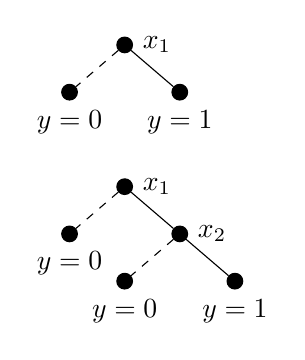
\begin{tikzpicture}
          \visible<2->{
            \node (1n1) [circle,draw,fill,inner sep=2pt,label=right:$x_1$] at (0,0) {};
            \node (1n2) [circle,draw,fill,inner sep=2pt,label={below:$y=0$}] at (-0.7,-0.6) {};
            \node (1n3) [circle,draw,fill,inner sep=2pt,label={below:$y=1$}] at (0.7,-0.6) {};
            \draw [dashed] (1n1) -- (1n2);
            \draw (1n1) -- (1n3);
          }

          \visible<3->{
            \node (1n1) [circle,draw,fill,inner sep=2pt,label=right:$x_1$] at (0,-1.8) {};
            \node (1n2) [circle,draw,fill,inner sep=2pt,label={below:$y=0$}] at (-0.7,-2.4) {};
            \node (1n3) [circle,draw,fill,inner sep=2pt,label={right:$x_2$}] at (0.7,-2.4) {};
            \node (1n4) [circle,draw,fill,inner sep=2pt,label={below:$y=0$}] at (0,-3.0) {};
            \node (1n5) [circle,draw,fill,inner sep=2pt,label={below:$y=1$}] at (1.4,-3.0) {};
            \draw [dashed] (1n1) -- (1n2);
            \draw (1n1) -- (1n3);
            \draw [dashed] (1n3) -- (1n4);
            \draw (1n3) -- (1n5);
          }
        \end{tikzpicture}
      \end{center}
    \end{column}
  \end{columns}
\end{frame}

\begin{frame}{Thesis Contribution}
  % Development of BiOptSat
  % Evaluation of 5 variants and comparison to two existing approaches
  \begin{itemize}
    \item Development of the \algname{} algorithm
    \item Implementation of the \algname{} algorithm and its competitors (will be released open source)
    \item Evaluation of variants of \algname{} and comparison to two competitors
    \item Evaluation of refinements to \algname{}
  \end{itemize}
\end{frame}

\begin{frame}{High-Level Overview of \algname{}}
  % Declarative approach to solving problems
  % Search progress of lexicographic method
  
\end{frame}

\begin{frame}{Results}
  % Cactus and MSH scatter

\end{frame}

\begin{frame}{Self-Reflection}
  % Start with a summer internship!
  
\end{frame}

{
\usebackgroundtemplate{
\transparent{0.3} % requires \usepackage{transparent} & compile twice
\setlength{\unitlength}{1cm}
\begin{picture}(16,9)
\put(0.2,1){
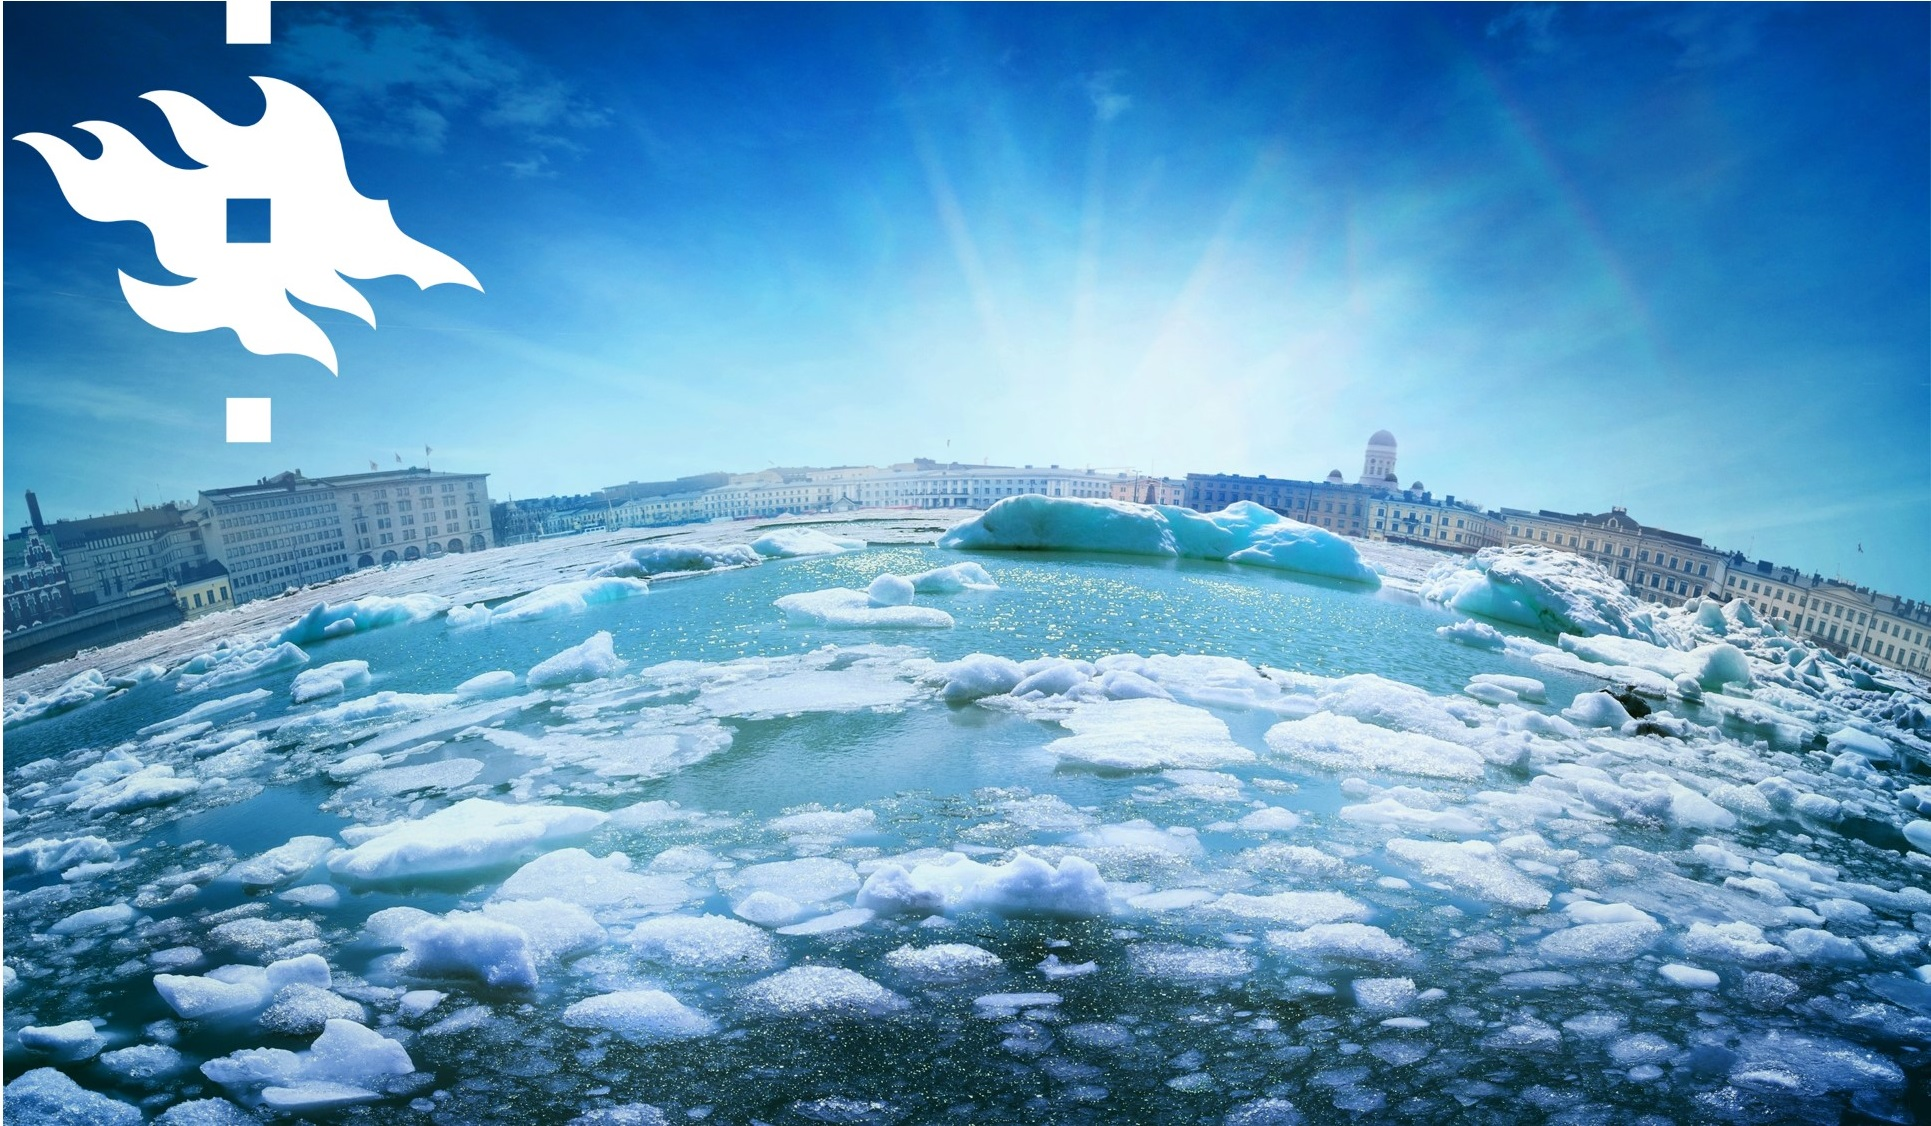
\includegraphics[width=15cm,height=7.5cm]{hy_brand_image_1_wide_background_hires_logo}
}
\end{picture}
\setlength{\unitlength}{1pt}
}

\begin{frame}
  \centering
  \Large
  Thank you for your attention!
\end{frame}
}

\appendix

\begin{frame}{Propositional Satisfiability}
  
\end{frame}

\begin{frame}{Maximum Satisfiability}
  
\end{frame}

\begin{frame}{\algname{}}
  \begin{algorithm}[H]
    \caption{\algname{}: MaxSAT-based bi-objective optimization}
    \textbf{Input}: A formula $\formula$, two objectives $\Obj_\inc$ and $\Obj_\dec$.\\
    \textbf{Output}: Either one or all pareto-optimal solution for each pareto point of $\formula$.

    \begin{algorithmic}[1]
      \STATE $\sol^r \gets \texttt{InitSATsolverAndSolve}(F)$ \quad\COMMENT{Invokes the SAT solver on the formula.}
      \STATE $b_\dec \gets \infty, b_\inc \gets 0$
      \WHILE{$\res = \text{SAT}$}
      \STATE $(b_\inc, \sol^r) \gets \Min(b_\dec , \Obj_\inc(\sol^r))$  \quad\COMMENT{Maintains $\tot(\Obj_\inc)$ (or similar)}
      \STATE $(b_\dec, \sol^r) \gets  \Simpr(b_\inc , \Obj_\dec(\sol^r))$  \quad\COMMENT{Builds $\tot(\Obj_\dec)$}
      \STATE \textbf{yield} $\sol^r$  \quad\COMMENT{Optionally:  \textbf{yield} $\E(b_\dec, b_\inc)$}
      \STATE $(\res, \sol^r) \gets \satsolver(\{\ov{\Obj_\dec}{b_\dec}\})$
      \ENDWHILE
    \end{algorithmic}
  \end{algorithm}
\end{frame}

\end{document}
